\documentclass{article}

\usepackage[utf8]{inputenc} % allow utf-8 input
\usepackage[T1]{fontenc}    % use 8-bit T1 fonts
\usepackage{hyperref}       % hyperlinks
\usepackage{url}            % simple URL typesetting
\usepackage{booktabs}       % professional-quality tables
\usepackage{amsfonts}       % blackboard math symbols
\usepackage{nicefrac}       % compact symbols for 1/2, etc.
\usepackage{microtype}      % microtypography
\usepackage{xcolor}         % colors
\usepackage{graphicx}       % figures
\graphicspath{{./}{final_report/}}

\title{Final Report - Project 7\\Sentiment Analysis}

\author{
  Group 19 \\
  Nolan Capomaggio and Mathis Morra-Fischer \\
}


\begin{document}


\maketitle

\begin{abstract}
This project studies binary sentiment classification on the Amazon Reviews
dataset. Reviews are classified as negative or positive using TF-IDF with
Logistic Regression, a configurable LSTM/BiLSTM neural network, and reduced
RoBERTa fine-tuning experiments. The final experiments focus on reproducibility,
dataset-size reduction, hyperparameter sensitivity, regularization, and
computational cost. Logistic Regression remains the strongest practical
baseline, reaching 94.07\% accuracy on the full test set. On a 100k-sample
experiment, Logistic Regression reaches 91.34\% test accuracy in 11.6 seconds,
while the best LSTM configuration reaches 90.71\% but requires around 9
minutes. The best reduced RoBERTa experiment reaches 94.25\% test accuracy on a
5k-sample setup, but requires substantially more runtime than Logistic
Regression.
\end{abstract}

\section{Introduction}
Sentiment analysis is a standard Natural Language Processing task where the
goal is to automatically detect the polarity of a text. In this project, we
work on binary sentiment classification of Amazon product reviews. The label
$0$ represents negative reviews and the label $1$ represents positive reviews.

The project compares methods of increasing complexity. Logistic Regression with
TF-IDF is used as a fast and interpretable baseline. LSTM models are used to
test whether sequence modeling improves performance. A RoBERTa pipeline is used
to evaluate whether partial transformer fine-tuning improves accuracy enough to
justify its additional cost.

\section{Dataset and Preprocessing}
We use the Amazon Reviews dataset from Kaggle by Adam Bittlingmayer. The
dataset is already formatted for fastText:
\begin{itemize}
  \item \texttt{\_\_label\_\_1}: negative review, mapped to class 0;
  \item \texttt{\_\_label\_\_2}: positive review, mapped to class 1.
\end{itemize}
The full dataset contains 3.6 million training reviews and 400,000 official test
reviews. The classes are balanced, so accuracy is a meaningful metric.

The training file is split into train and validation subsets using a stratified
80/20 split. This preserves the 50/50 class balance. All experiments use seed
42 unless otherwise stated. The code fixes Python, NumPy, and PyTorch random
seeds, and passes the seed to the model-specific training components.

The shared preprocessing removes HTML tags, lowercases the text, and normalizes
whitespace. Punctuation is kept because it may carry sentiment information.

\section{Implemented Methods}
\subsection{Logistic Regression with TF-IDF}
The baseline uses a \texttt{scikit-learn} pipeline composed of:
\begin{itemize}
  \item TF-IDF vectorization with unigrams and bigrams;
  \item a maximum vocabulary size of 100,000 features;
  \item \texttt{min\_df=2} to remove very rare terms;
  \item sublinear term-frequency scaling;
  \item Logistic Regression with $\ell_2$ regularization and $C=1.0$.
\end{itemize}

This approach does not model long-distance word order, but it is very efficient
on large text datasets and gives a strong reference point.

\subsection{LSTM / BiLSTM}
The LSTM implementation contains:
\begin{itemize}
  \item a vocabulary built from the training set;
  \item integer encoding and padding/truncation to a fixed sequence length;
  \item an embedding layer;
  \item one or more LSTM layers, optionally bidirectional;
  \item global max pooling over the sequence dimension;
  \item dropout;
  \item a final linear classifier.
\end{itemize}

The model is trained with Adam and cross-entropy loss. We added several
hyperparameters to support final experiments: learning rate, embedding size,
hidden size, number of layers, bidirectionality, dropout, weight decay, frozen
embedding layer, and seed-controlled data loading. The training script writes a
\texttt{metrics.json} file and, for neural models, a
\texttt{training\_history.json} file.

\subsection{RoBERTa}
The RoBERTa pipeline uses the Hugging Face Transformers library with
\texttt{roberta-base}. It supports full fine-tuning, freezing the first $N$
encoder layers, or freezing the whole encoder and training only the
classification head. Because full fine-tuning is expensive, the final RoBERTa
experiments freeze a large part of the encoder and fine-tune only the upper
transformer layers plus the classification head. This makes RoBERTa feasible on
the available laptop while still allowing the model to adapt to the sentiment
task.

\section{Experimental Protocol}
We evaluate models with accuracy, macro F1-score, macro precision, and macro
recall. Runtime is also recorded because the professor specifically asked us to
compare whether additional complexity improves accuracy enough to justify the
computation time.

The experiments are organized around the following questions:
\begin{itemize}
  \item How much can the dataset be reduced while still obtaining useful
  performance?
  \item Does LSTM improve over Logistic Regression?
  \item How sensitive is LSTM to the learning rate?
  \item Does increasing model capacity improve results?
  \item Do dropout and weight decay reduce overfitting or improve accuracy?
\end{itemize}

\section{Results}
\subsection{Dataset Reduction with Logistic Regression}
Table~\ref{tab:logreg-data} shows that Logistic Regression performs well even
with a small fraction of the training set.

\begin{table}[h]
  \centering
  \caption{Logistic Regression results when reducing the training set size.}
  \label{tab:logreg-data}
  \begin{tabular}{rrrr}
    \toprule
    Loaded train examples & Test examples & Test accuracy & Runtime (s) \\
    \midrule
    2,000 & 2,000 & 0.8145 & 4.25 \\
    10,000 & 5,000 & 0.8698 & 2.27 \\
    100,000 & 20,000 & 0.9134 & 11.57 \\
    Full dataset & 400,000 & 0.9407 & 465.00 \\
    \bottomrule
  \end{tabular}
\end{table}

\begin{figure}[h]
  \centering
  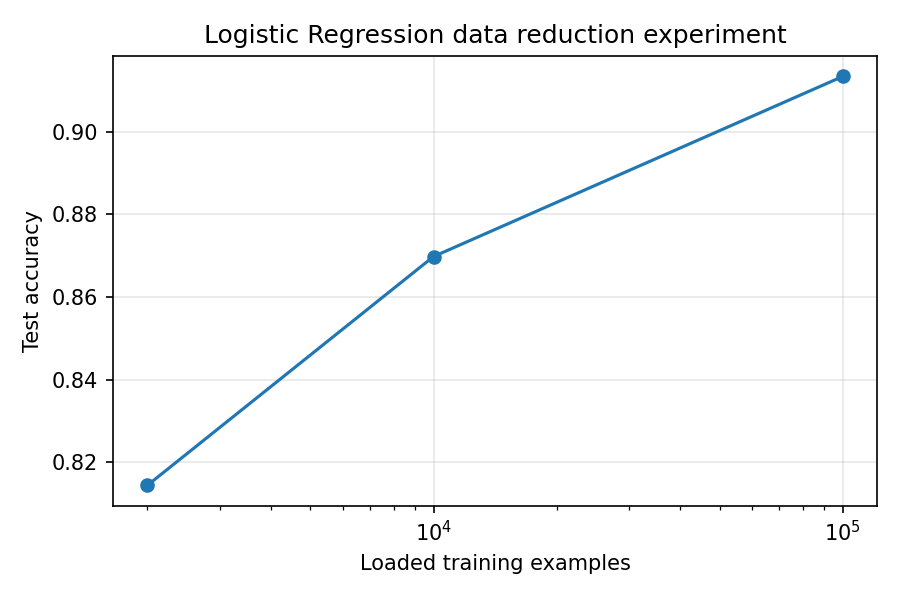
\includegraphics[width=0.72\linewidth]{logistic_data_curve.png}
  \caption{Effect of training-set size on Logistic Regression test accuracy.}
  \label{fig:logreg-data}
\end{figure}

The first important finding is that only 2,000 loaded training examples already
give 81.45\% test accuracy. This is above the 70--80\% threshold discussed at
the midterm. Increasing the dataset to 100,000 examples improves accuracy to
91.34\%, and the full-dataset run reached 94.07\% in 465 seconds.

\subsection{LSTM Hyperparameter Experiments}
All LSTM experiments below use 100,000 loaded training examples, 20,000 test
examples, 3 epochs, seed 42, and sequence length 256.

\begin{table}[h]
  \centering
  \small
  \caption{LSTM experiment results.}
  \label{tab:lstm-results}
  \begin{tabular}{lrrrr}
    \toprule
    Configuration & Test accuracy & Macro F1 & Val accuracy & Runtime (s) \\
    \midrule
    BiLSTM, lr=$10^{-3}$ & 0.9071 & 0.9069 & 0.9104 & 535.09 \\
    BiLSTM, lr=$10^{-4}$ & 0.8018 & 0.8001 & 0.8007 & 529.24 \\
    BiLSTM, 3 layers & 0.9070 & 0.9068 & 0.9093 & 1599.01 \\
    BiLSTM, dropout=0.5 & 0.8963 & 0.8959 & 0.8967 & 528.18 \\
    BiLSTM, weight decay=$10^{-4}$ & 0.9014 & 0.9010 & 0.9023 & 535.75 \\
    \bottomrule
  \end{tabular}
\end{table}

\begin{figure}[h]
  \centering
  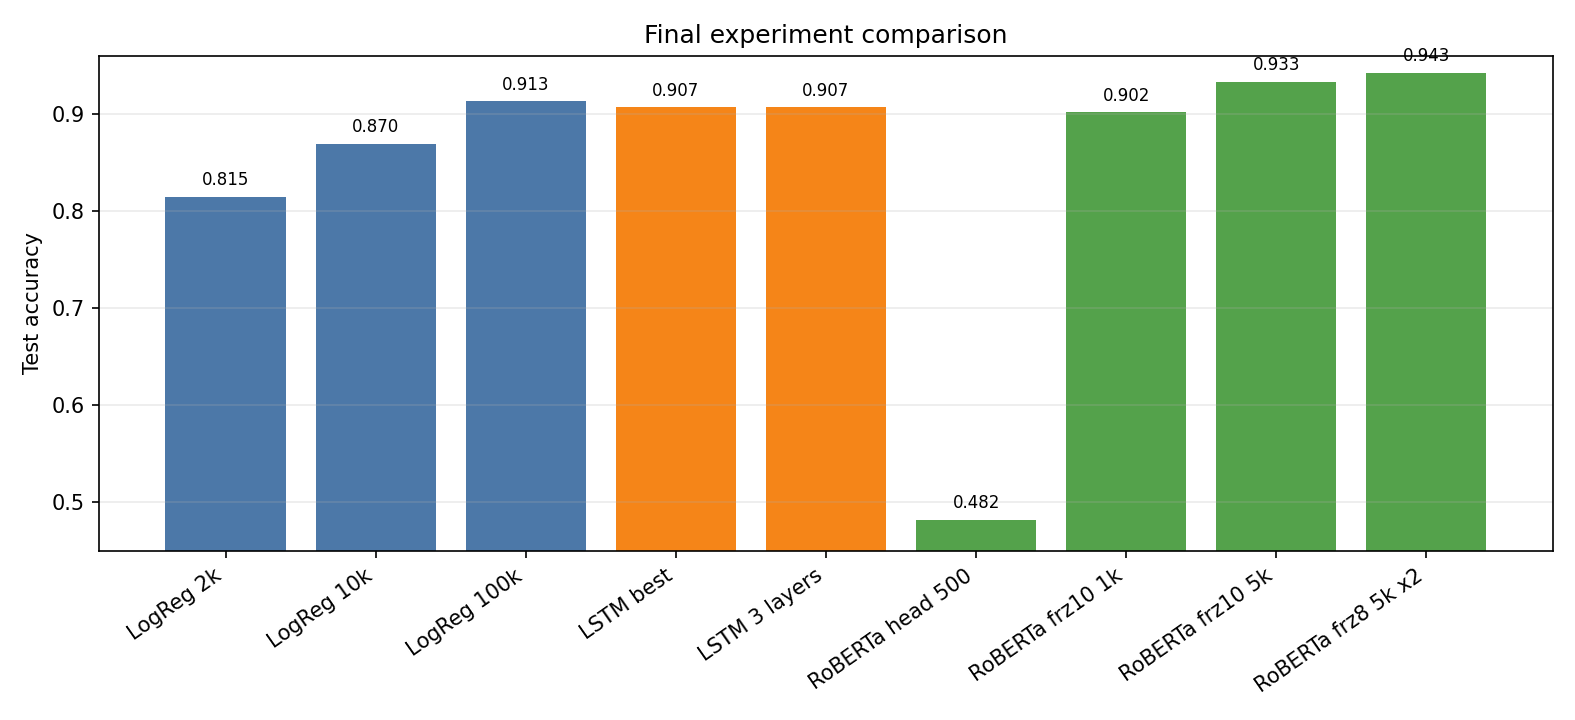
\includegraphics[width=0.92\linewidth]{experiment_accuracy_comparison.png}
  \caption{Comparison of selected Logistic Regression, LSTM, and RoBERTa experiments.}
  \label{fig:accuracy-comparison}
\end{figure}

\subsection{RoBERTa Experiments}
Table~\ref{tab:roberta-results} shows the reduced RoBERTa experiments. The
first run freezes the whole encoder and trains only the classification head.
The later runs unfreeze the top transformer layers, which gives the model
enough capacity to adapt to the sentiment task.

\begin{table}[h]
  \centering
  \caption{Reduced RoBERTa fine-tuning results.}
  \label{tab:roberta-results}
  \small
  \begin{tabular}{lrrrrr}
    \toprule
    Configuration & Train & Test & Epochs & Test accuracy & Runtime (s) \\
    \midrule
    Head only & 500 & 500 & 1 & 0.4820 & 35.35 \\
    Freeze 10 layers & 1,000 & 1,000 & 1 & 0.9020 & 70.22 \\
    Freeze 10 layers & 5,000 & 2,000 & 1 & 0.9330 & 270.53 \\
    Freeze 8 layers & 5,000 & 2,000 & 1 & 0.9380 & 352.34 \\
    Freeze 8 layers & 5,000 & 2,000 & 2 & 0.9425 & 707.03 \\
    \bottomrule
  \end{tabular}
\end{table}

The head-only run is close to random guessing. This is expected because the
classification head starts from random weights while the frozen encoder cannot
adapt to the task. Once the upper transformer layers are unfrozen, RoBERTa
improves sharply. With 5,000 loaded training examples, freezing the first 8
layers and training for 2 epochs reaches 94.25\% test accuracy, the best result
among our reduced experiments.

\begin{figure}[h]
  \centering
  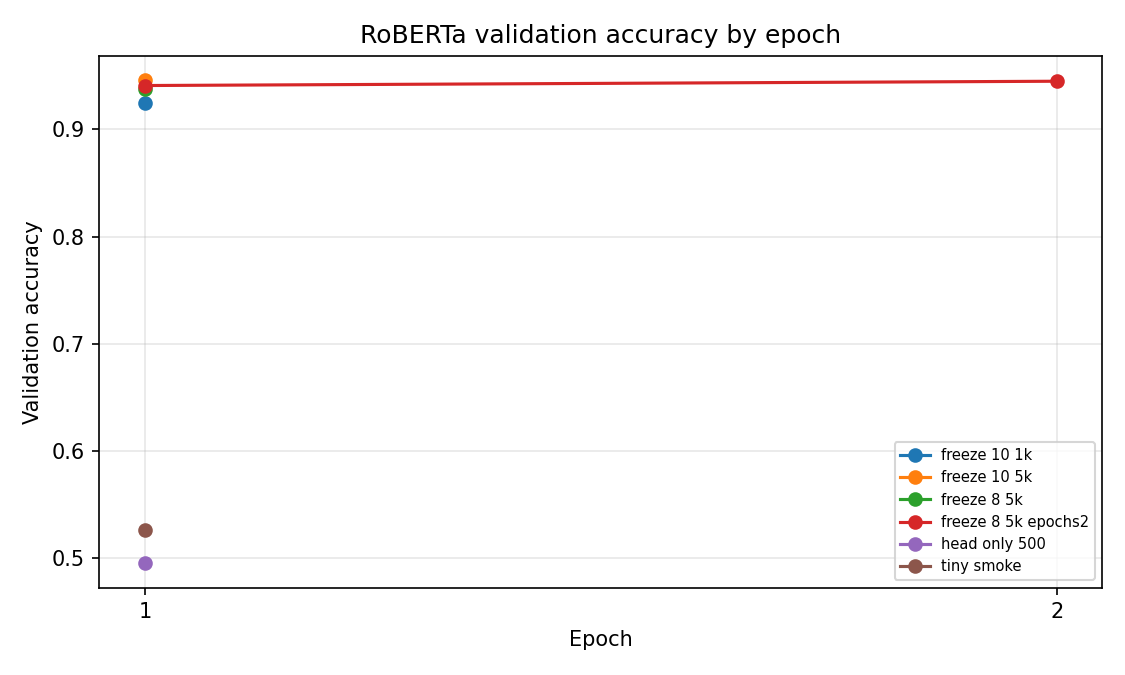
\includegraphics[width=0.78\linewidth]{roberta_validation_curves.png}
  \caption{Validation accuracy curves for the RoBERTa experiments.}
  \label{fig:roberta-curves}
\end{figure}

\begin{figure}[h]
  \centering
  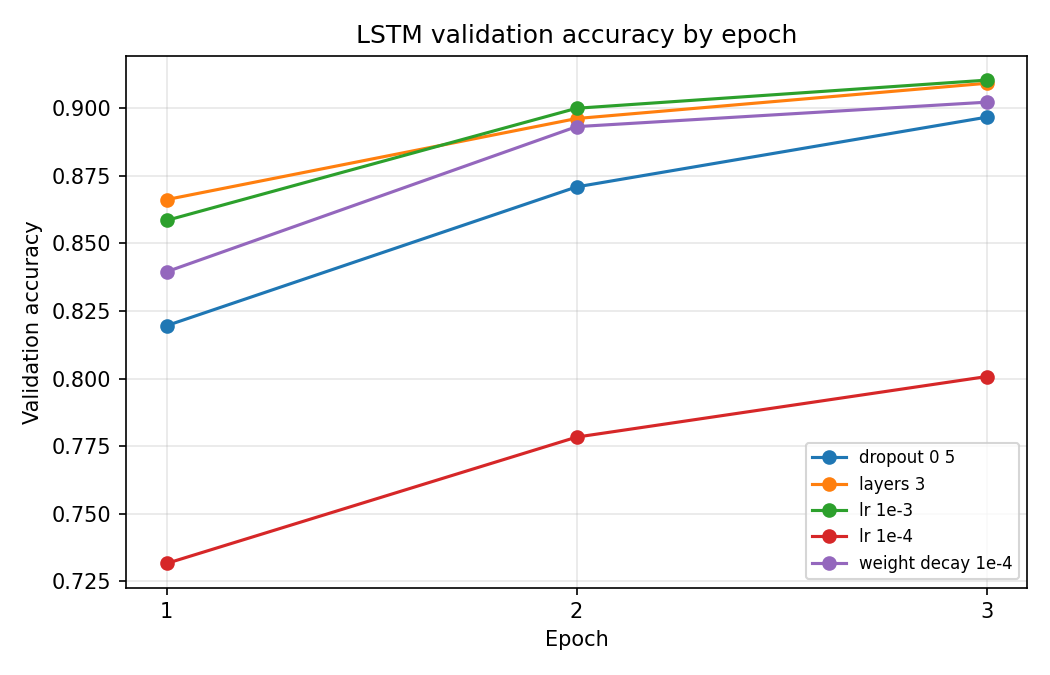
\includegraphics[width=0.78\linewidth]{lstm_validation_curves.png}
  \caption{Validation accuracy curves for the LSTM experiments.}
  \label{fig:lstm-curves}
\end{figure}

\section{Discussion}
\subsection{Learning Rate}
The learning rate has a strong effect on LSTM performance. With
$lr=10^{-3}$, the model reaches 90.71\% test accuracy. With $lr=10^{-4}$, the
test accuracy drops to 80.18\%. The validation history shows that the smaller
learning rate is still improving after 3 epochs, so the problem is likely
undertraining rather than overfitting. A lower learning rate may require more
epochs to converge.

\subsection{Model Capacity}
Increasing the LSTM from 1 layer to 3 layers does not improve test accuracy:
90.70\% versus 90.71\%. Runtime increases from about 535 seconds to 1599
seconds. This is a clear negative result: extra depth increases compute time
without meaningful accuracy gain. It may also increase optimization difficulty
and risk of overfitting if trained longer.

\subsection{Regularization}
Increasing dropout from 0.3 to 0.5 reduces test accuracy from 90.71\% to
89.63\%. Adding weight decay of $10^{-4}$ reaches 90.14\%, also below the
baseline LSTM. In these runs, stronger regularization did not improve the final
score. The baseline LSTM does not show strong overfitting after 3 epochs because
validation accuracy continues to improve while training loss decreases.

\subsection{Logistic Regression vs LSTM}
The most important conclusion is that Logistic Regression is still the best
accuracy/time trade-off. On the 100k experiment, Logistic Regression reaches
91.34\% test accuracy in 11.57 seconds. The best LSTM reaches 90.71\% but takes
around 535 seconds. Therefore, on this dataset, the additional sequence-modeling
capacity of LSTM does not justify its computational cost.

This result is explainable. Amazon sentiment reviews often contain strong local
lexical cues such as ``great'', ``bad'', ``waste of money'', or ``not good''.
TF-IDF with bigrams captures many of these patterns efficiently. LSTM can model
word order, but the gain is limited because the dataset is large and the
baseline features are already very informative.

\subsection{RoBERTa Trade-off}
RoBERTa becomes the strongest reduced-data model once upper layers are unfrozen.
The best RoBERTa run reaches 94.25\% test accuracy with only 5,000 loaded
training examples, which is higher than Logistic Regression on 100,000 loaded
examples. However, this comes at a much higher computational cost: the 2-epoch
RoBERTa run takes 707 seconds, compared with 11.57 seconds for Logistic
Regression on 100,000 examples. This shows that transformer fine-tuning can
improve accuracy, but the improvement must be weighed against runtime and
hardware requirements.

\section{Limitations}
RoBERTa was evaluated only on reduced subsets, not on the full dataset. This
means the reported RoBERTa result should be interpreted as a strong reduced-data
experiment, not as a full benchmark of the transformer model. Full fine-tuning
on the complete dataset would likely require more memory and more time than was
available on the laptop.

Another limitation is that we did not perform a full grid search. Instead, we
selected targeted experiments based on the midterm feedback: dataset reduction,
learning rate, model depth, dropout, and weight decay.

\section{Conclusion}
The final project implemented a complete reproducible sentiment classification
pipeline and compared classical and neural approaches. Logistic Regression with
TF-IDF is a very strong baseline: it reaches 94.07\% accuracy on the full test
set in 465 seconds, and already reaches 91.34\% with only 100,000 loaded
training examples.

The LSTM experiments show that neural sequence models are sensitive to
hyperparameters. A learning rate of $10^{-3}$ works much better than
$10^{-4}$ for 3 epochs. Adding layers, dropout, or weight decay did not improve
the result in our experiments. The best LSTM reaches about 90.71\% test
accuracy, slightly below Logistic Regression on the same 100k setup while being
much slower.

RoBERTa gives the best reduced-data accuracy when partially unfrozen, reaching
94.25\% with 5,000 loaded training examples. The main conclusion is therefore
more nuanced: Logistic Regression gives the best performance-cost trade-off,
while RoBERTa gives the best accuracy in our reduced experiments but requires
significantly more compute. More complex models must be justified not only by
accuracy, but also by runtime, hardware requirements, and practical usefulness.

\end{document}
